\section{User Interface Representation (Of  Respective Project)}

The applications interface is designed for retinal image enhancement, the functionality is implemented using matlab, and the phase of testing the product was accomplished successfully. The application can very well manage by the medical staff .
Also doctors can detect the early disease in a human body using enhanced retinal image delivered by our project .
  



\subsection{Snapshots of system}


\begin{figure}[ht]
\centering
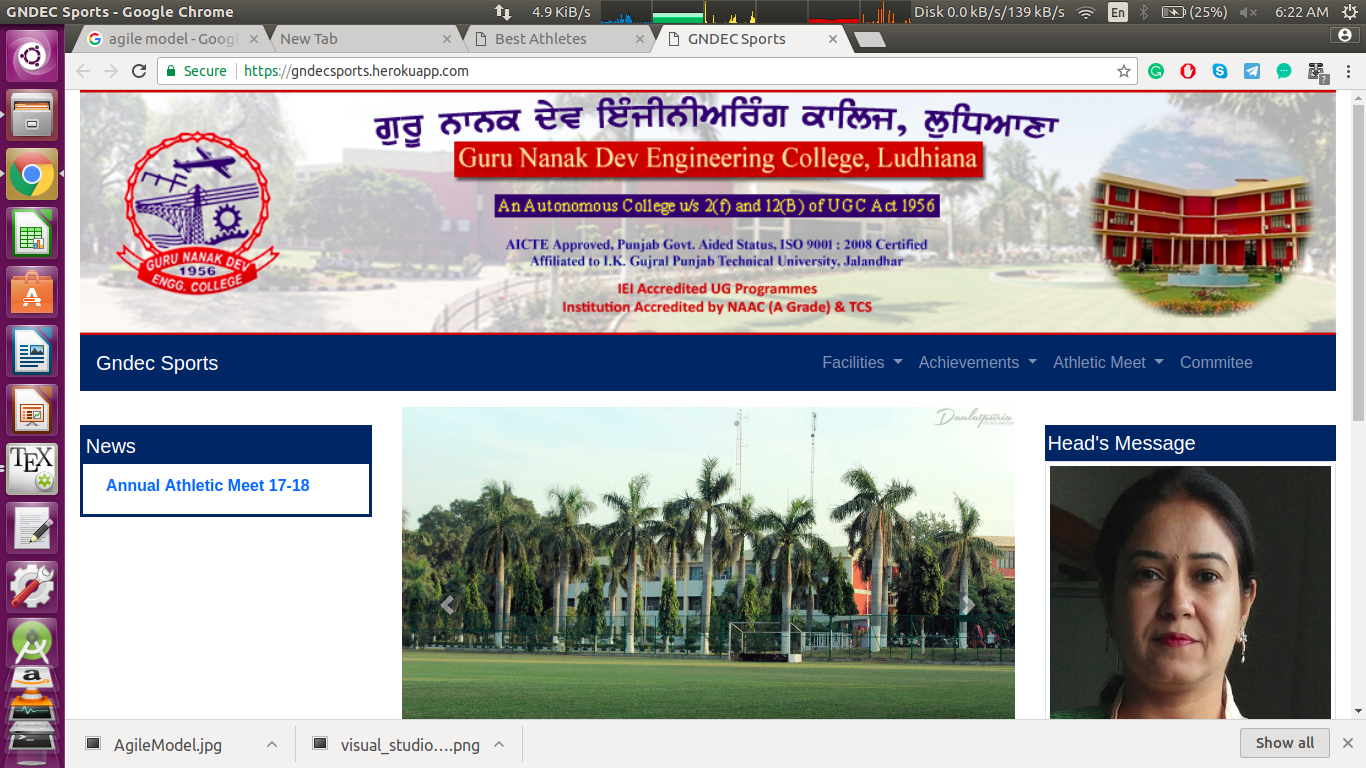
\includegraphics[scale=0.28]{images/HomeUserHeroku.png}
\caption{Home Screen}
\end{figure}

\newpage
\begin{figure}[ht]
\centering
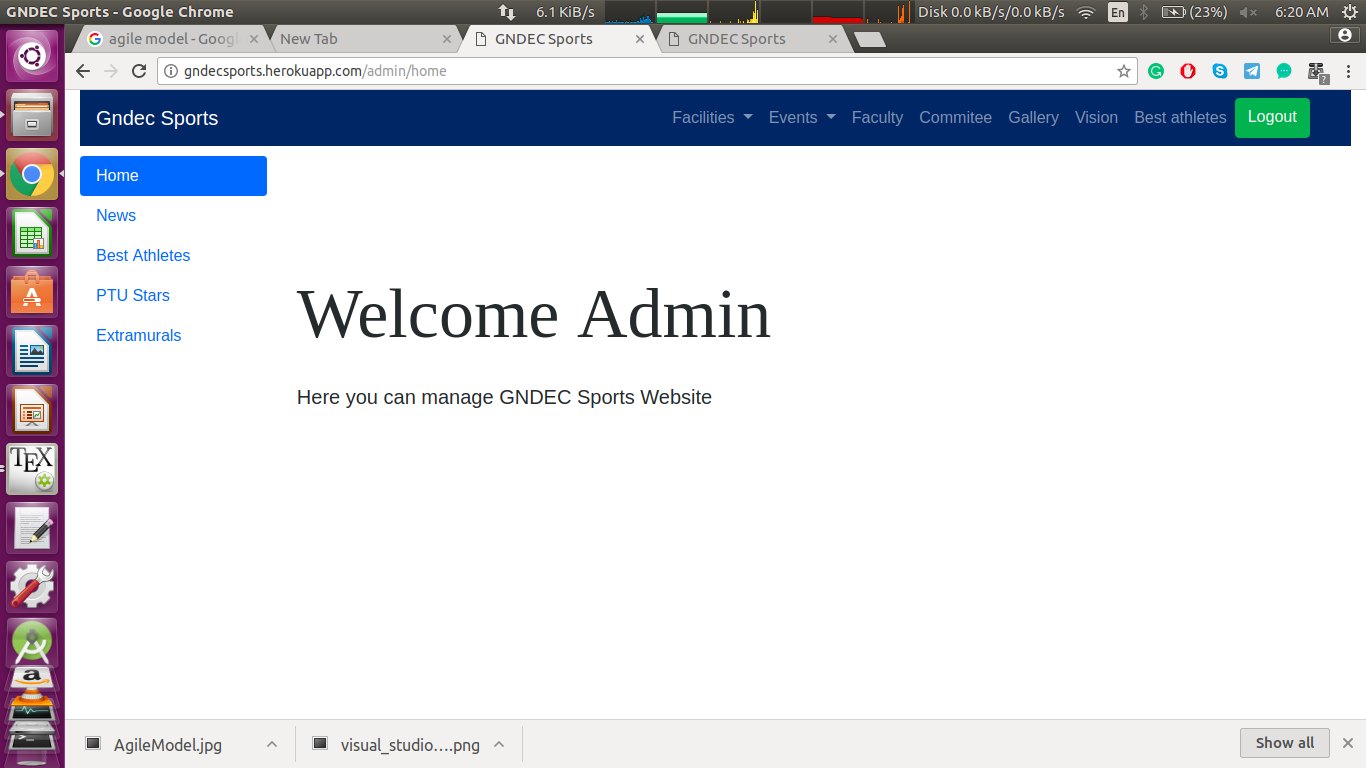
\includegraphics[scale=0.35]{images/HomeAdminHeroku.png}
\caption{Home Screen (Admin)}
\end{figure}

\newpage

\begin{figure}[ht]
\centering
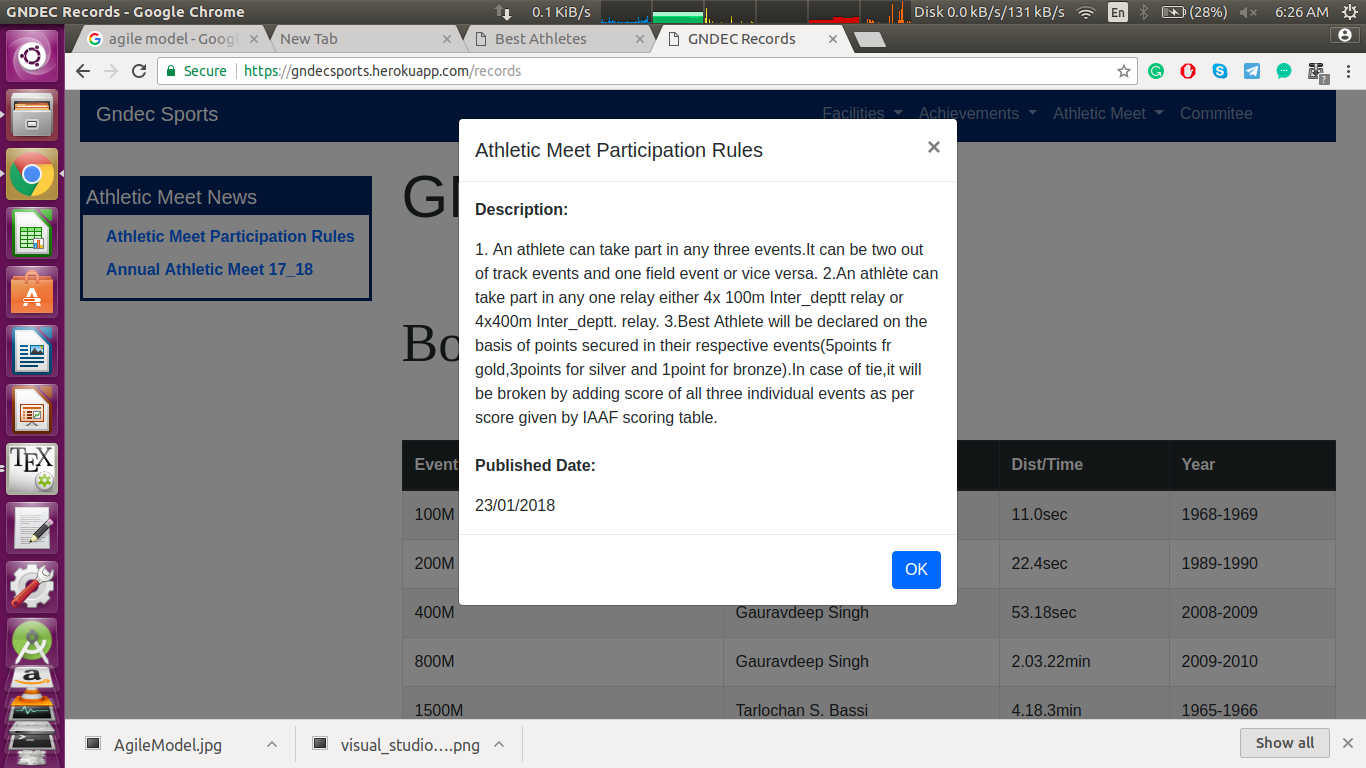
\includegraphics[scale=0.35]{images/NewsPanelHeroku.png}
\caption{News Panel}
\end{figure}

\newpage

\begin{figure}[ht]
\centering
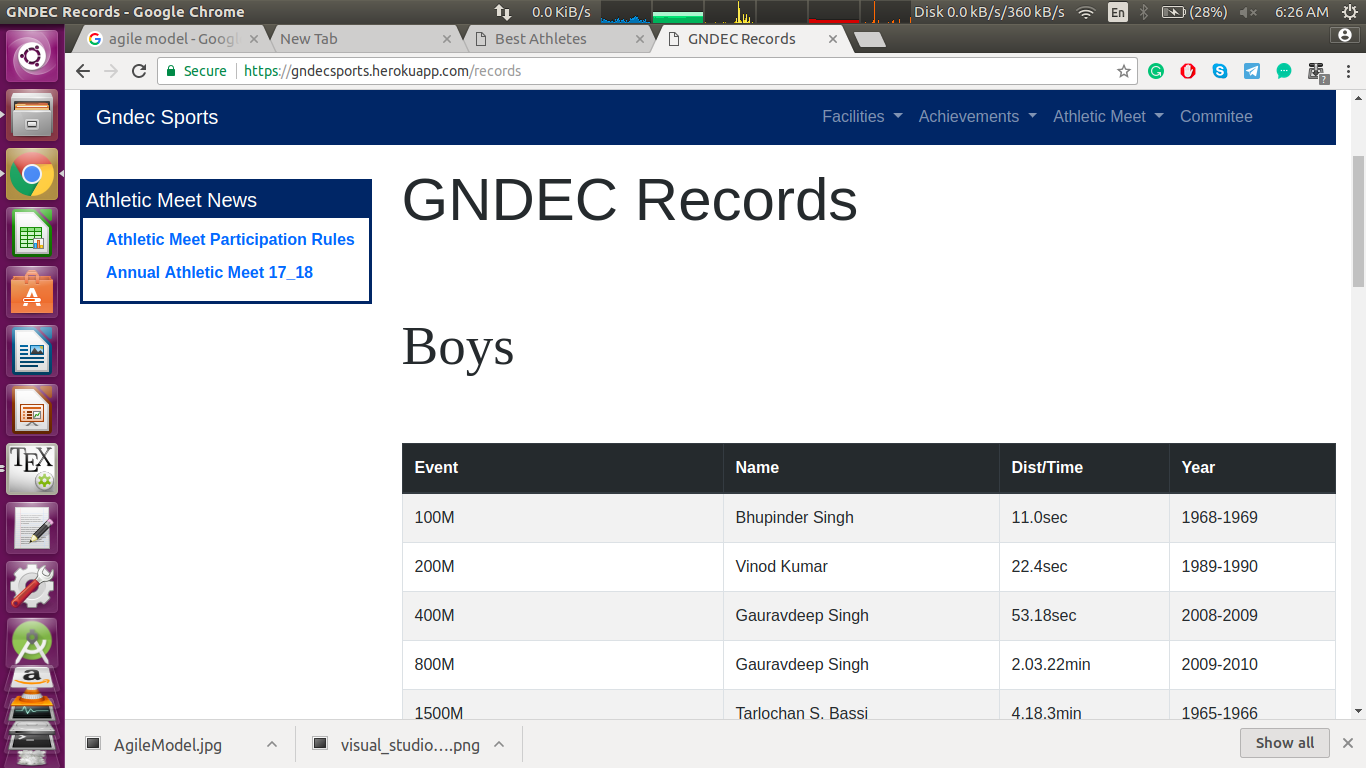
\includegraphics[scale=0.35]{images/RecordsHeroku.png}
\caption{Records}
\end{figure}

\newpage

\begin{figure}[ht]
\centering
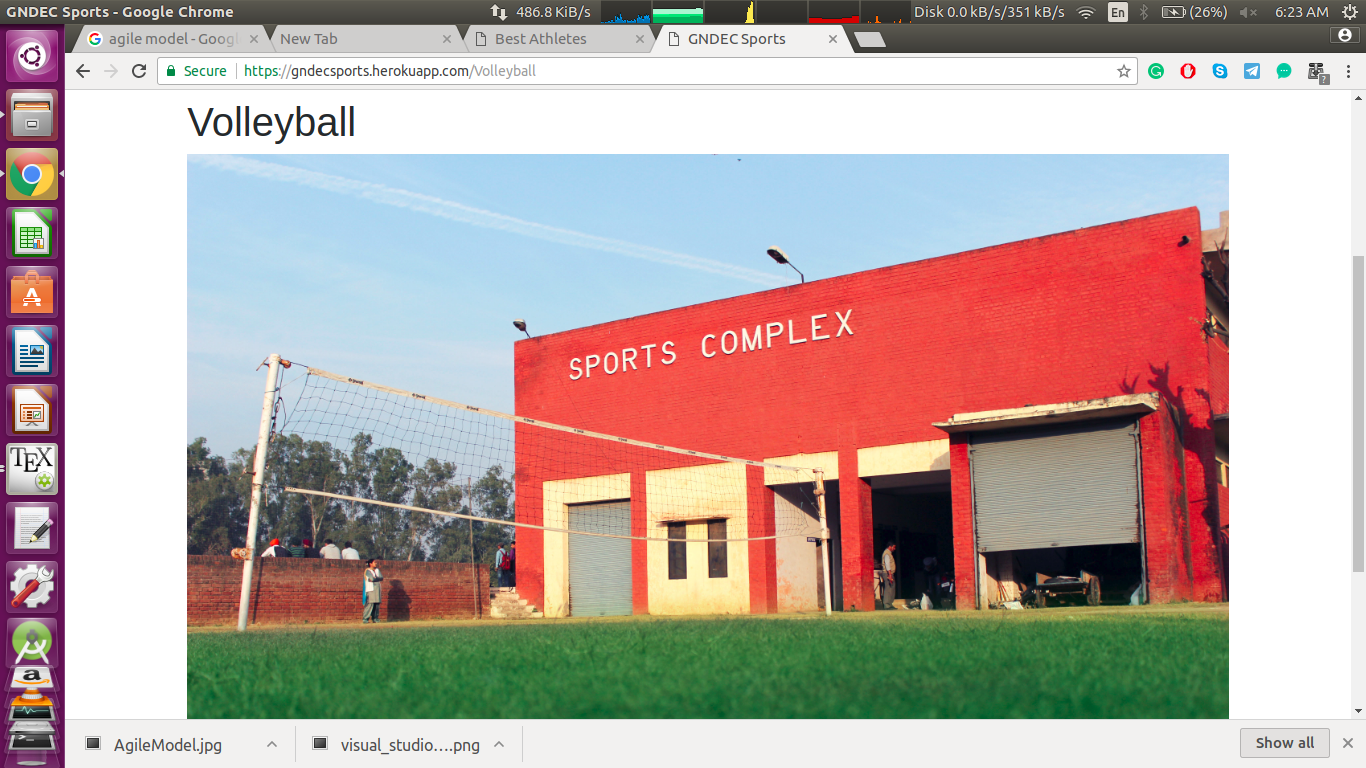
\includegraphics[scale=0.35]{images/VollyballHeroku.png}
\caption{Facilities}
\end{figure}

\newpage

\begin{figure}[ht]
\centering
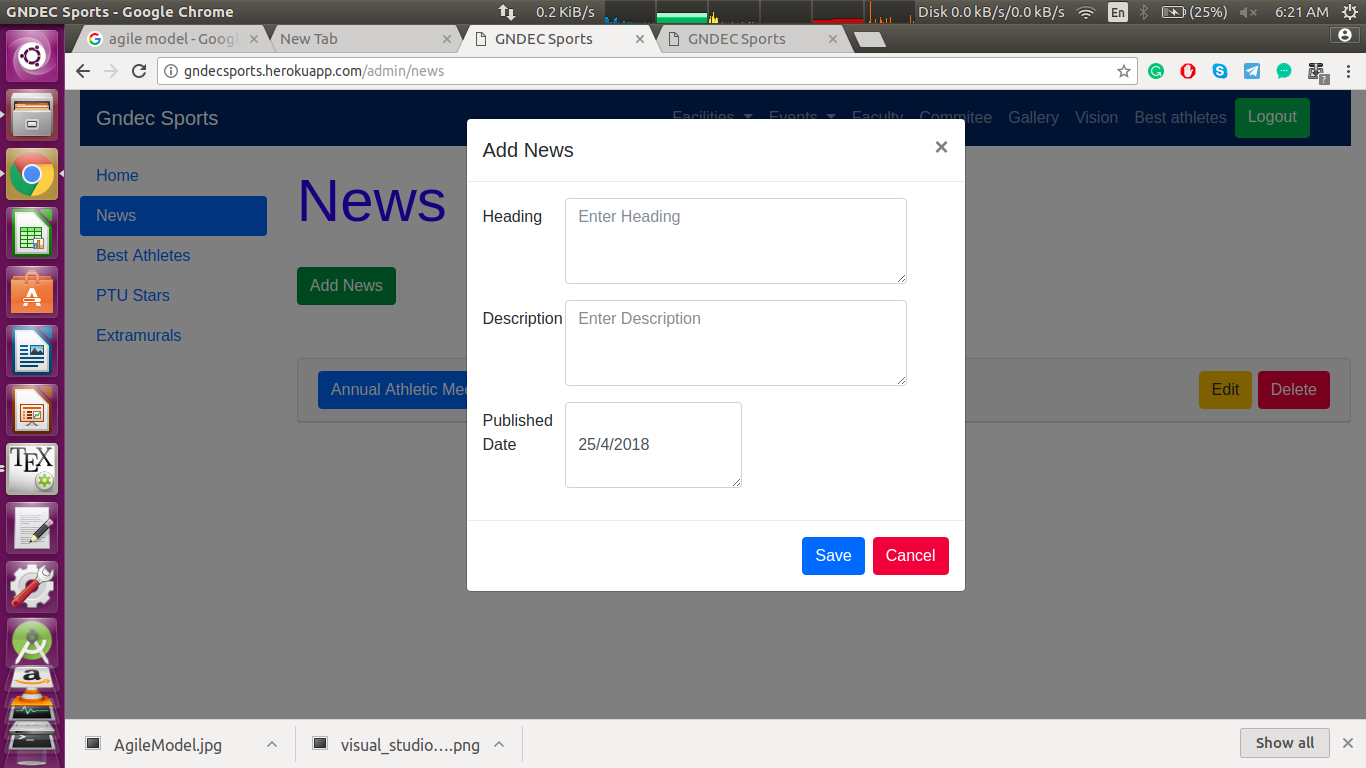
\includegraphics[scale=0.35]{images/AddNewsHeroku.png}
\caption{Add News Panel}
\end{figure}

\newpage

\begin{figure}[ht]
\centering
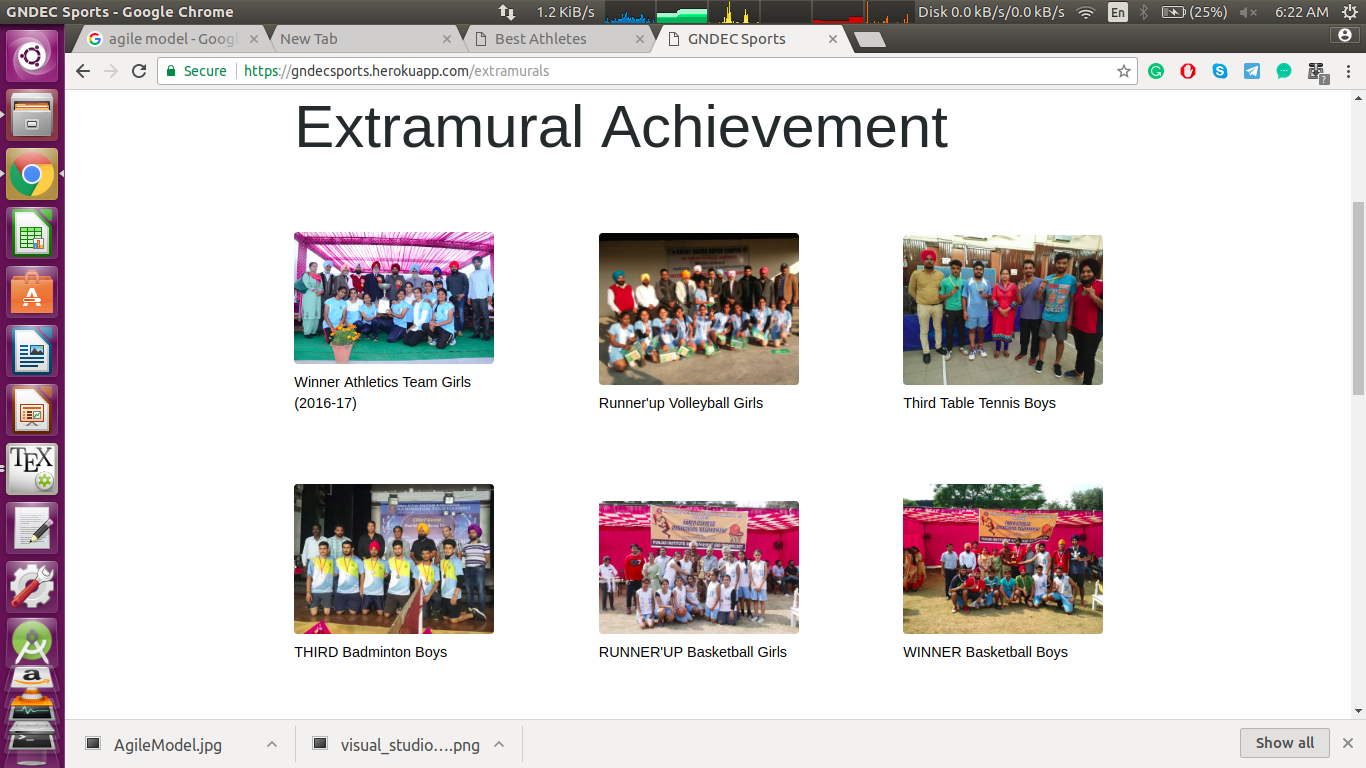
\includegraphics[scale=0.35]{images/AchievementHeroku.png}
\caption{Achievements}
\end{figure}

\newpage

\begin{figure}[ht]
\centering
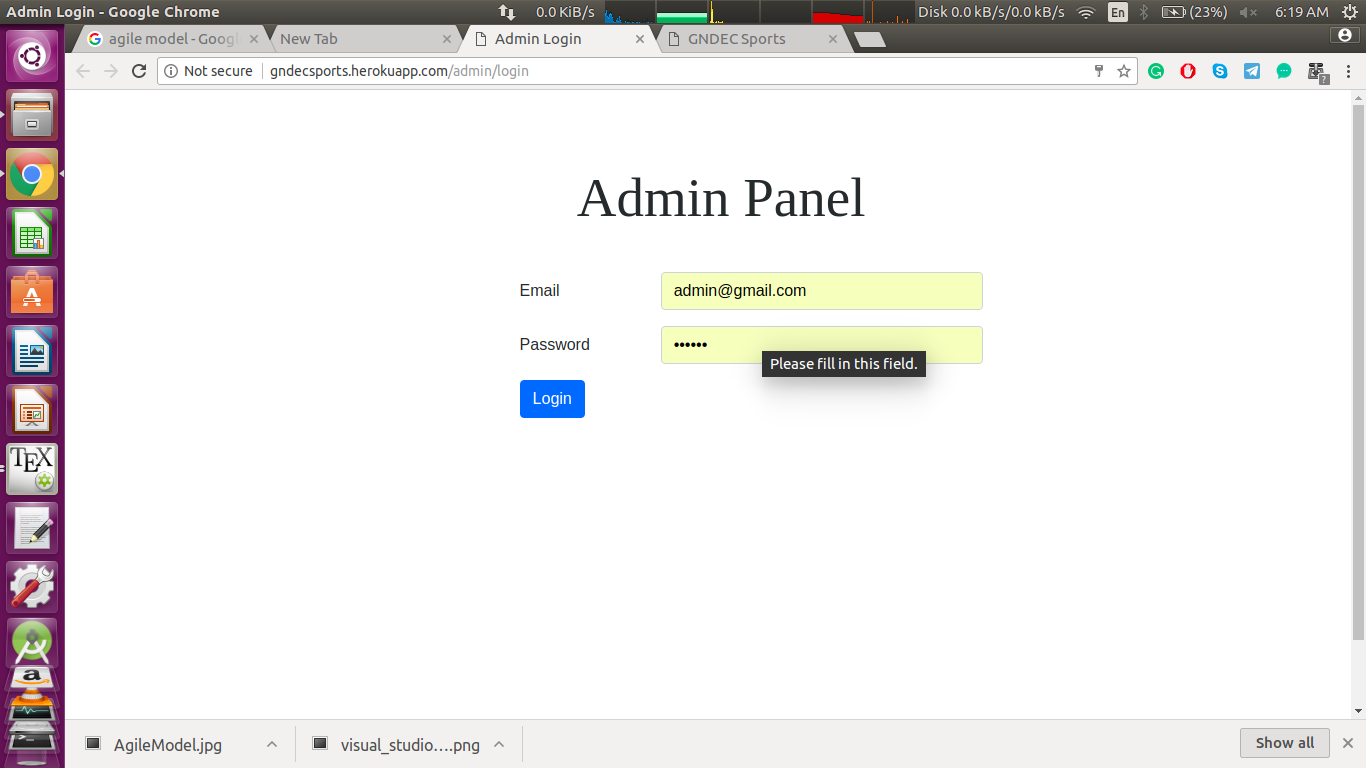
\includegraphics[scale=0.35]{images/AdminPanelHeroku.png}
\caption{Admin Login Panel}
\end{figure}

\newpage

\begin{figure}[ht]
\centering
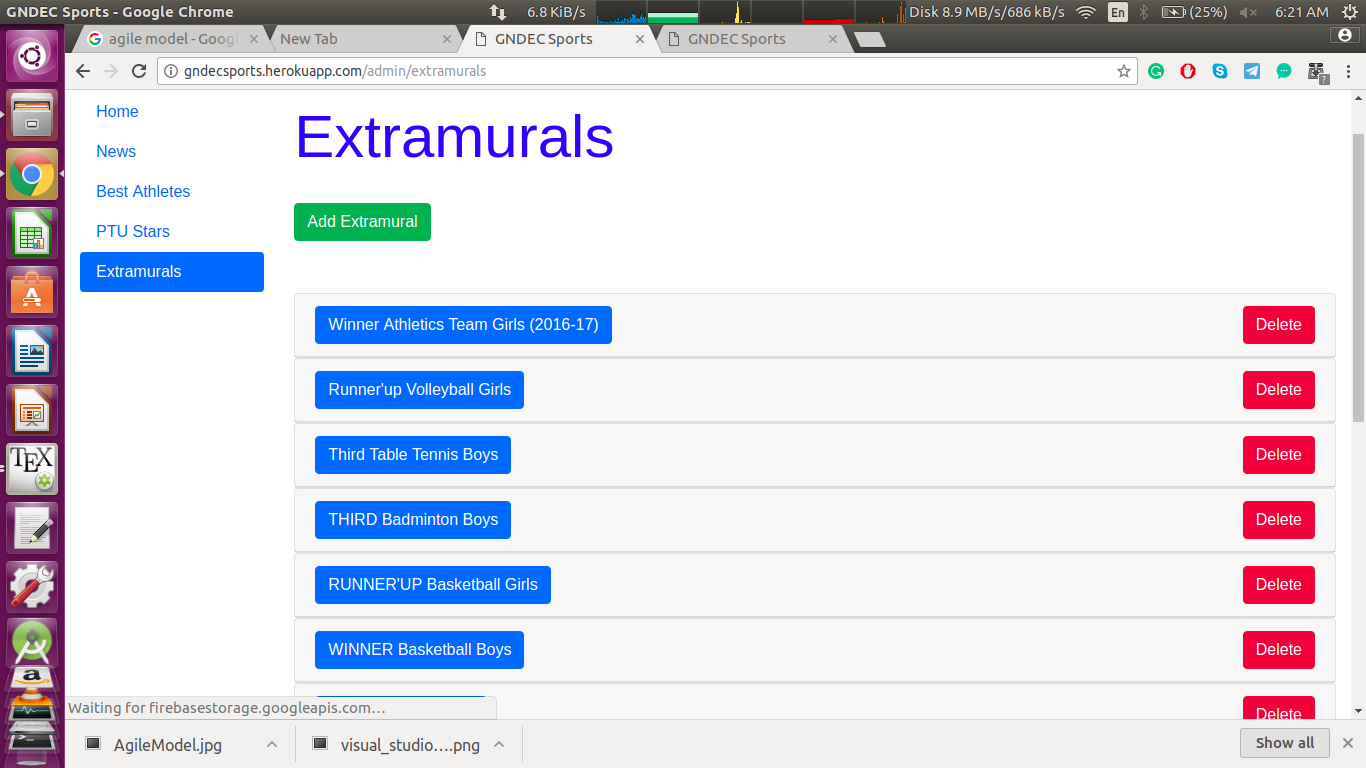
\includegraphics[scale=0.35]{images/ExtramuralHeroku.png}
\caption{Extramural}
\end{figure}


\newpage
\section{Back Ends Representation (Database to be used)}
\subsection{DRIVE}
The photographs for the DRIVE database were obtained from a diabetic retinopathy screening program in The Netherlands. The screening population consisted of 400 diabetic subjects between 25-90 years of age. Forty photographs have been randomly selected, 33 do not show any sign of diabetic retinopathy and 7 show signs of mild early diabetic retinopathy. Each image has been JPEG compressed.

The images were acquired using a Canon CR5 non-mydriatic 3CCD camera with a 45 degree field of view (FOV). Each image was captured using 8 bits per color plane at 768 by 584 pixels. The FOV of each image is circular with a diameter of approximately 540 pixels. For this database, the images have been cropped around the FOV. For each image, a mask image is provided that delineates the FOV.

\subsection{How does it work?}

The set of 40 images has been divided into a training and a test set, both containing 20 images. For the training images, a single manual segmentation of the vasculature is available. For the test cases, two manual segmentations are available; one is used as gold standard, the other one can be used to compare computer generated segmentations with those of an independent human observer. All human observers that manually segmented the vasculature were instructed and trained by an experienced ophthalmologist. They were asked to mark all pixels for which they were for at least 70 percent certain that they were vessel.

All of the images contained in the database were actually used for making clinical diagnoses. To ensure the utmost protection of patient privacy, information that might allow the identity of a patient to be reconstructed has been removed, and we have no actual knowledge that the images could be used alone or in combination to identify any subject. To minimize any further risk of breach of privacy, the use of this database is restricted to those individuals or organizations that obtained the database directly from this website.

\newpage
\subsection{Snapshots of Database}
\begin{figure}[ht]
		\centering
		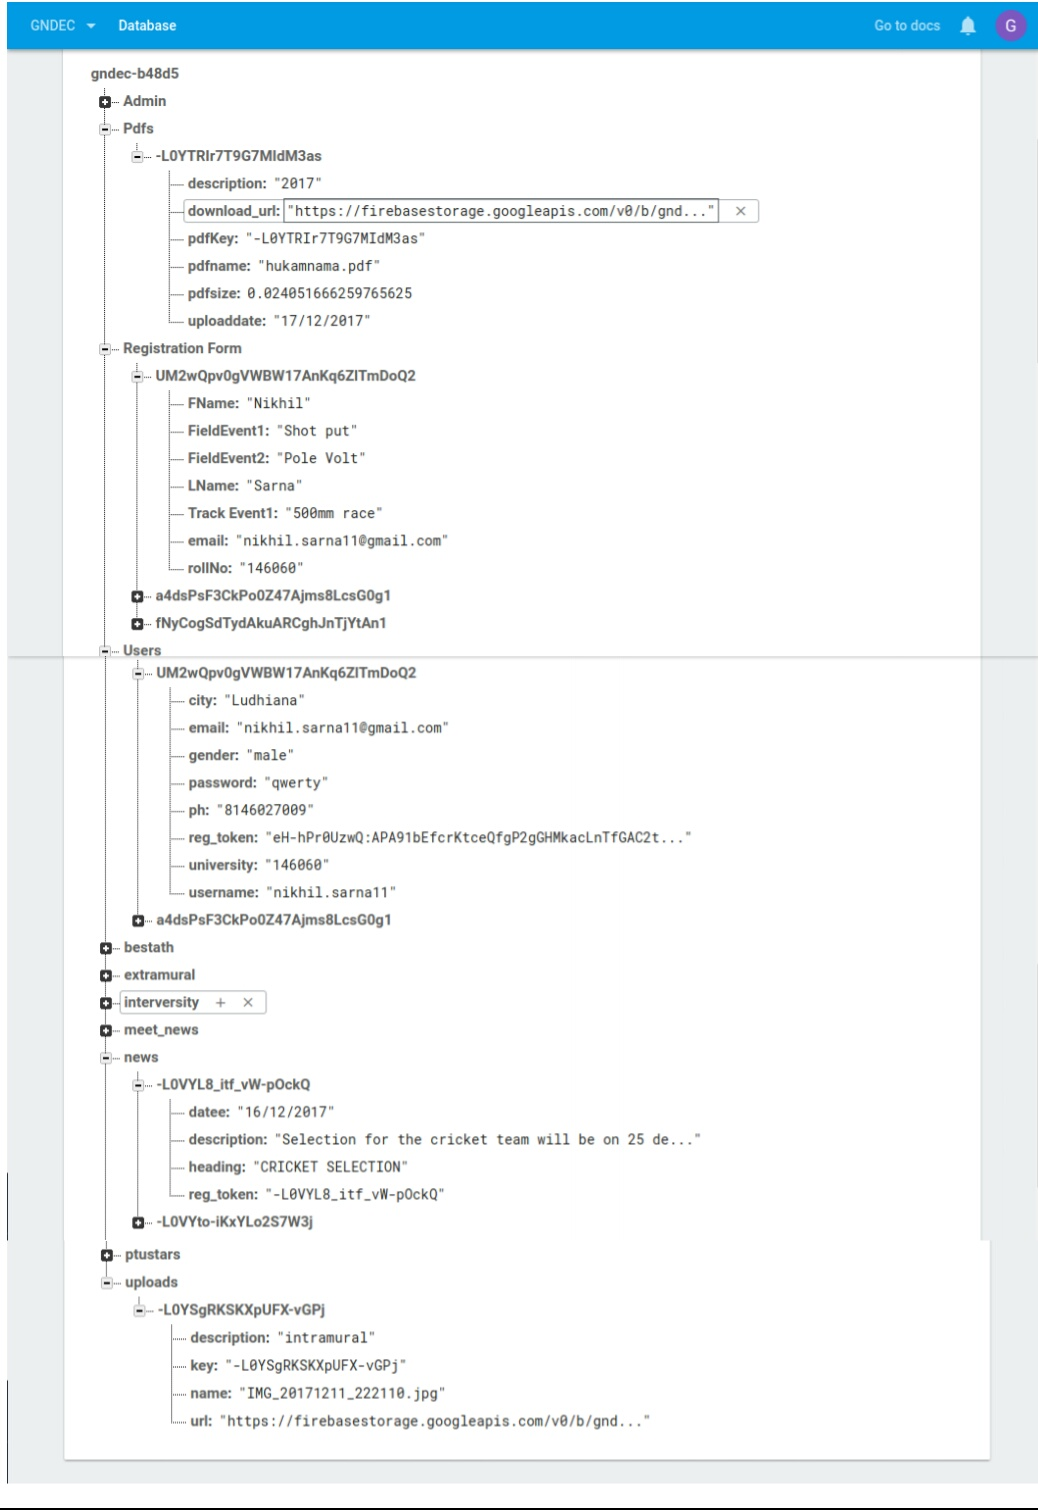
\includegraphics[scale=0.30]{images/dbfire.jpg}
		\caption{Database}
	\end{figure}



